\apendice{Plan de Proyecto Software}

\section{Introducción}

\section{Planificación temporal}

\subsection{Planificación por \textit{sprints}}


\subsubsection{\textit{Sprint 1:}}

\begin{itemize}
	\item \textbf{\textit{Planning meeting}}
	
	Durante la reunión se marcaron los siguientes objetivos:
	
	\begin{enumerate}
		\item Configuración básica: incluyendo la creación del repositorio, la correcta instalación de ZenHub, la creación de entornos virtuales (miniconda, SKLearn, etc.) y la familiarización con conceptos \textit{scrum}: \textit{milestones, sprints, epics}, etc.
		
		\item Memoria: comienzo de la redacción incluyendo las secciones de introducción, conceptos teóricos (aprendizaje automático) y trabajo relacionado.
		
		\item Investigación: búsqueda del código SSADR-CoF y de las bases de datos utilizadas en el paper.
		
		\item Lectura de papers: Engelen y Hoos~\cite{engelen2020surveyOnSemiSupervised}, García, Triguero y Herrera~\cite{triguero2015SelflabeledTechniques}, y Zhou y Duan~\cite{zhou2021SemisupervisedRecommendationAttack}.
	\end{enumerate}
	
	\item \textbf{Marcas temporales}
	
	El sprint se desarrolló entre el 24 de septiembre de 2022 y el 2 de octubre del 2022.
	
	\item \textbf{\textit{Burndown Report}}
	
	\begin{figure}[h]
		\caption{\textit{Burndown Report Sprint 01}}
		\centering
		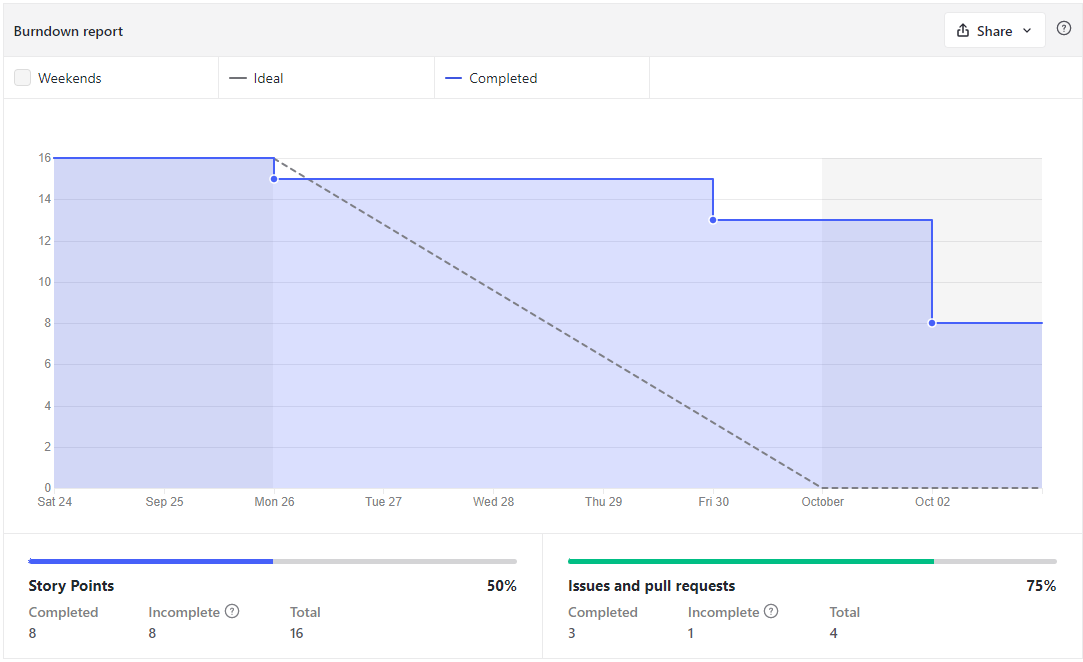
\includegraphics[width=\textwidth]{../img/anexos/s01_bdr}
	\end{figure}
	
	Como se puede comprobar, no todos los objetivos marcados fueron cumplidos: la estimación del tiempo fue demasiado optimista, además de no contar con el tiempo requerido en solucionar problemas técnicos (\LaTeX{}). Se dejó para próximos sprints la lectura del último paper.
	
	\item \textbf{\textit{Sprint review meeting}}
	Durante la reunión se fijaron ciertas correcciones en la memoria (mejorar referencias bibliográficas y la sección de <<Trabajos relacionados>>), además de la necesidad de introducir una sección teórica de ataques a los sistemas de recomendación.
	
	
\end{itemize}


\subsubsection{\textit{Sprint 2:}}

\begin{itemize}
	\item \textbf{\textit{Planning meeting}}
	
	Objetivos del siguiente Sprint:
	
	\begin{enumerate}
		
		\item Configuración: debido a la gran cantidad de tiempo invertida en solucionar errores de compilación en \LaTeX{}, se decidió migrar el proyecto a una nueva instalación basada en Debian.
		\item Correcciones: aspectos estilísticos y completar información.
		\item Lectura: Mingdan y Qingshan~\cite{mingdan2018ShillingAttacksAReview} con el objetivo de introducir una sección teórica de ataques.
		\item Memoria: redacción completa de los modelos de ataque en los aspectos teóricos.
		
	\end{enumerate}
	
	\item \textbf{Marcas temporales}
	
	El sprint se desarrolló entre el 03 de octubre de 2022 y el 18 de octubre del 2022.
	
	\item \textbf{\textit{Burndown Report}}
	
	\begin{figure}[h]
		\caption{\textit{Burndown Report Sprint 02}}
		\centering
		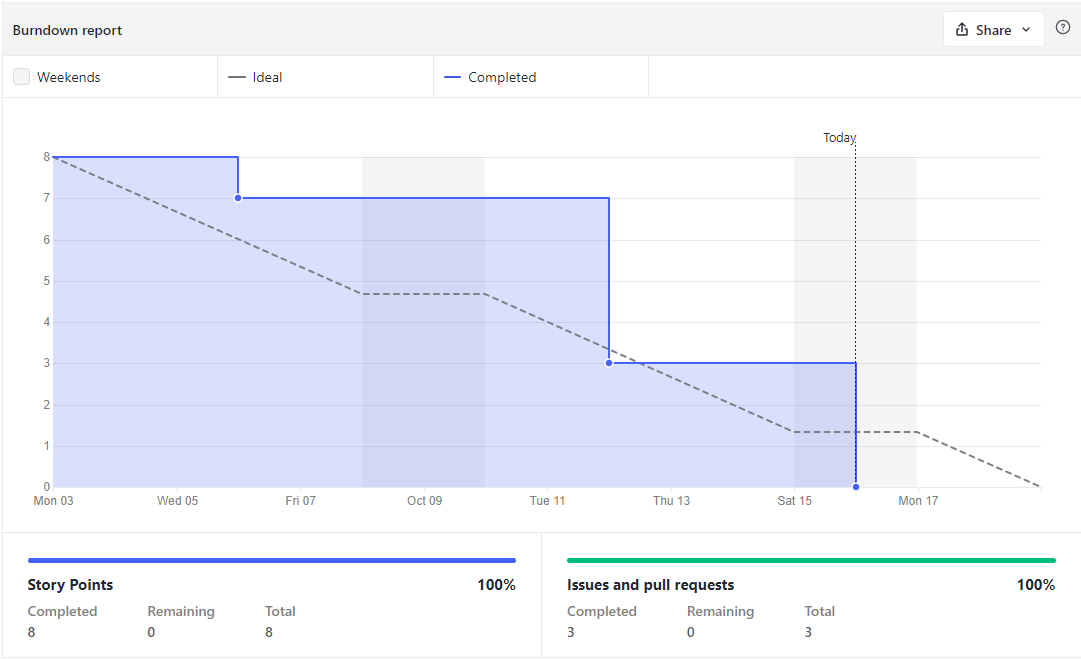
\includegraphics[width=\textwidth]{../img/anexos/s02_bdr}
	\end{figure}
		
	En este Sprint sí se cumplió con los objetivos marcados. Sin embargo, la estimación de tiempo tampoco fue la adecuada, requiriendo más de lo previsto.
	
	\item \textbf{\textit{Sprint review meeting}}
	
\end{itemize}


\subsubsection{\textit{Sprint N:}}
\begin{itemize}
	\item \textbf{\textit{Planning meeting}}
	\item \textbf{Marcas temporales}		
	\item \textbf{\textit{Burndown Report}}
	\item \textbf{\textit{Sprint review meeting}}
\end{itemize}

\section{Estudio de viabilidad}

\subsection{Viabilidad económica}

\subsection{Viabilidad legal}


